\chapter{Kvalitetssikring}\label{ch:Kvalitetssikring}

I dette afsnit er det set på, hvordan gruppen har kvalitetssikret projektet. Der er taget udgangspunkt i parametre fra FURPS+ og praktikker fra XP. Disse praktikker skal fungere i harmoni med SCRUM, så kvaliteten af applikationen ikke tilsidesættes. Kvaliteten kan beskrives som værende primært ikke-funktionelle krav.

\section{FURPS+}

Som nævnt tidligere fokuserer agile udviklingsmetoder knap så meget på dokumentation, men mere på selve udviklingen af softwaren. Alt dokumentation, som ikke har en direkte indflydelse på softwaren, bliver nedprioriteret. Kvalitet i softwareudvikling omhandler koden mere end det gør andet. Kvalitetssikring kan beskrives ud fra FURPS+\cite{furps}. FURPS står for Functionality, Usability, Reliability, Performance og Supportability. Hvor Functionality omhandler de funktionelle krav, så beskriver URPS de ikke-funktionelle krav. 
Usability omhandler bruger-oplevelsen (User Experience) - hvordan brugeren skal interagere med systemet for en optimal oplevelse og forståelse. Til dette kan brugergrænsefladen designes så den er intuitiv og responsiv, samt nem at navigere. 
Reliability omhandler sikkerhed til at systemet skal kunne håndtere fejl og uhensigtmæssig brugeradfærd.
Performance omhandler responstid, tidsmål, og effektivitet af programmet. Dette ses som regel implementeret i form af Threads, og Async/Await og refaktorering af kode.
Supportability omhandler vedligehold, videreudvikling og konfigurering. Dette ses ofte i form af dokumentation af funktionaliteten af programmet, decoupling af klasser og interfaces.
I dette projekt er der lavet refaktorering, som er omskrivning af kode med henblik på at optimere koden eller forståelsen af koden. Dette gør det nemmere at vedligeholde som nævnt under FURPS. 
%Probably needs more than just refactoring

\section{XP praktikker}
Udover principperne fra FURPS, har praktikkerne fra XP også være en central del af projektet. Gruppen har tidligere besluttet at benytte procedurer fra XP til udviklingen af dette projekt, så procedurer som Pair Programming, Simple Design, Refactoring og Planning Game har gruppen sørget for at kvalitetssikre produktet. Til dette har Pair Programming og Test Driven Development\cite{Sommerville} haft en stor indflydelse på kvaliteten af produktet, da det øger Reliability og Supportability.
Under er der eksempler af hvordan teamet har benyttet procedurer fra XP til at kvalitetssikre produktet. 

\begin{figure}
    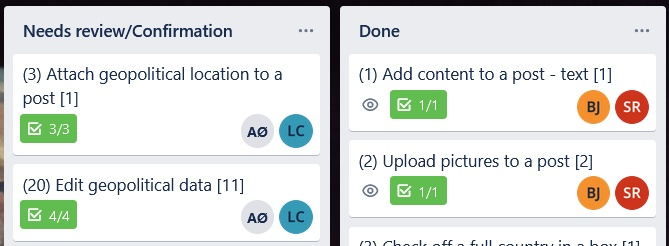
\includegraphics[width=\linewidth]{figures/pairprogramming.jpg}
    \caption{Ekempel af hvordan gruppen har benyttet Pair Programming fra XP.}
    \label{fig:Pair}
\end{figure}
% Bit of text here


\begin{figure}
    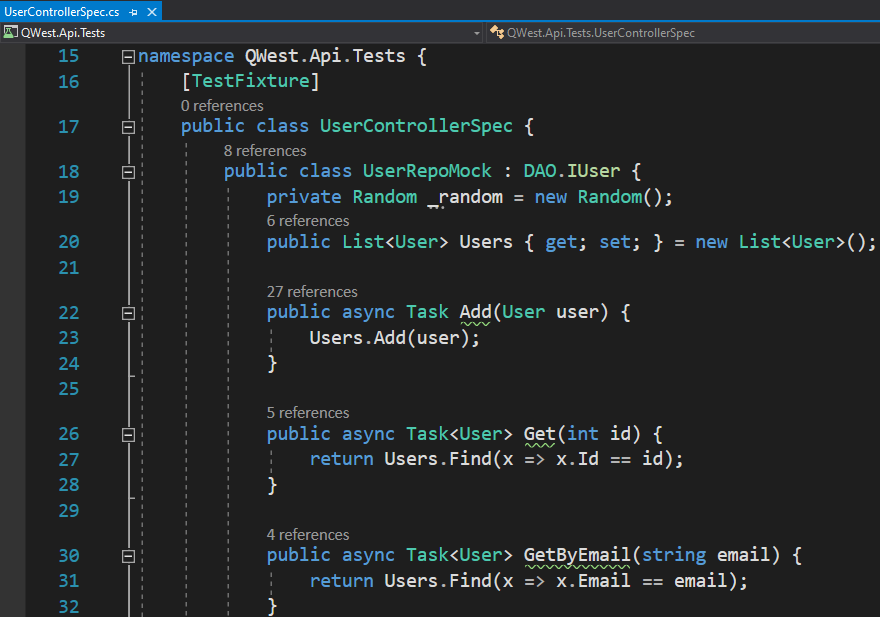
\includegraphics[width=\linewidth]{figures/tests.png}
    \caption{Eksempel på test.}
    \label{fig:Test}
\end{figure}
% Bit of text here
% Think we should primarily talk about our tests in Programming report

\begin{figure}
    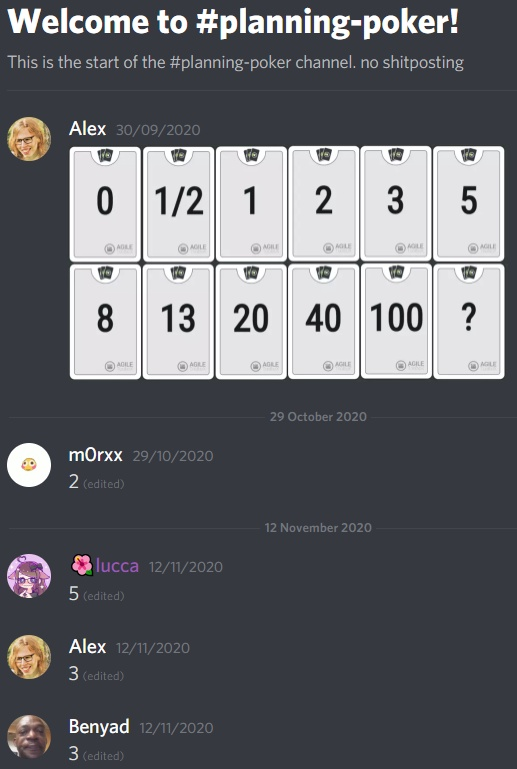
\includegraphics[width=\linewidth]{figures/planningpoker.jpg}
    \caption{Ekempel på hvordan Planning Poker er benyttet gennem hele projektet.}
    \label{fig:Poker}
\end{figure}
% Bit of text here